\section{Durchführung}
\label{sec:Durchführung}

\subsection*{Reflexionsgesetz}

Mithilfe des in \autoref{fig:abb3} dargestellten Aufbaus wird ein grüner Laserstrahl auf einen Spiegel gerichtet und anschließend der Einfallswinkel $\alpha_1$ sowie der Ausfallswinkel $\alpha_2$ anhand
der aufgedruckten Skala abgelesen. Dabei sollen sieben Einfallswinkel mit ihren korrespondierenden Ausfallswinkeln bestimmt werden.

\begin{figure}
    \centering
    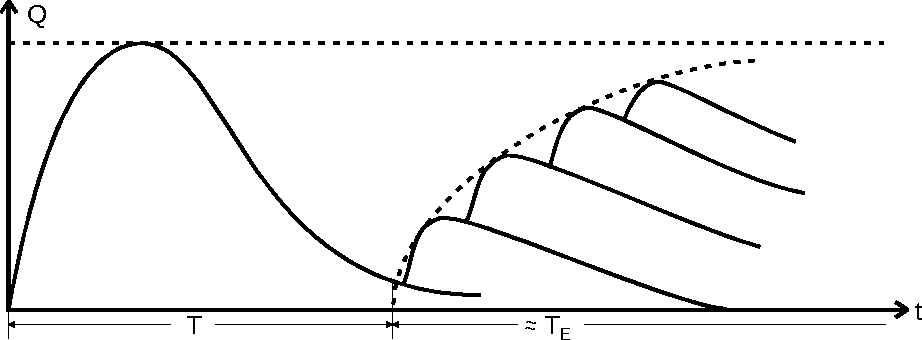
\includegraphics{figures/Abb_3.pdf}
    \caption{Abbildung des verwendeten Versuchaufbaus\cite{ap02}.}
    \label{fig:abb3}
\end{figure}

\subsection*{Brechungsgesetz}

Anstelle des zuvor verwendeten Spiegels (s. \autoref{fig:abb3}) wird nun eine planparallele Platte eingesetzt.
Es werden anhand der auf der planparallelen Platte aufgedruckten Skala zu sieben verschiedenen Einfallswinkeln $\alpha$ die Brechungswinkel $\beta$ abgelesen.


\subsection*{Ablenkungsgesetz}

Die planparallele Platte wird durch ein Prisma ersetzt.
Es werden sowohl für den grünen, als auch den roten Laser zu fünf verschiedenen Einfallswinkeln $\alpha_1$ im Bereich $10° \leq \alpha_1 \leq 60°$ die Austrittswinkel $\alpha_2$ bestimmt.


\subsection*{Beugungesetz}

Das Prisma wird durch ein Beugungsgitter ausgetauscht.
Um die verwendete Winkelskala wird ein Transmissionsschirm gelegt, sodass ein direktes Ablesen der Ablenkwinkel $\delta$ möglich ist.
Für den grünen und roten Laser werden die Beugungsmaxima zunächst für ein Gitter mit $d = \frac{1}{600} \, \unit{\milli\meter}$, dann für Gitter mit $d = \frac{1}{300} \, \unit{\milli\meter}$ und
$d = \frac{1}{100} \, \unit{\milli\meter}$ abgelesen.
